% BEGIN PREAMBEL
\documentclass[9pt]{beamer}
\usepackage[british]{babel}
\usepackage[latin1]{inputenc}
\usepackage{multimedia}
\usepackage{amsmath,amsfonts,amssymb}
\usepackage{upgreek}
\usepackage{pgfpages}
\usepackage[version=3]{mhchem}
\usepackage{lmodern}
\usepackage{graphicx}
\usepackage{multicol}
\usepackage{color}
\usepackage{xcolor}
\usepackage{wrapfig}
\usepackage{siunitx}
\usepackage{fontspec}
\newfontfamily\ubuntu{Ubuntu}
\newcommand{\as}{\\[14pt]}
\newcommand{\s}{\\[7pt]}
\newcommand{\is}{\\[2pt]}
\newcommand{\no}{\noindent}
\newcommand{\ka}{\hspace*{0.5cm}}
\newcommand{\ma}{\hspace*{1cm}}
\newcommand{\ga}{\hspace*{1.5cm}}
\newcommand{\li}{\left|}
\newcommand{\re}{\right|}
\newcommand{\const}{\text{const.}}
\newcommand{\z}{\text}
\newcommand{\terminal}[1]{\colorbox{black}{\textcolor{white}{{\fontfamily{phv}\selectfont \scriptsize{#1}}}}}
\newcommand{\plugin}[1]{\textit{\flq#1\frq}}
\definecolor{darkcerulean}{rgb}{0.03, 0.27, 0.49}
\newcommand{\ubu}[1]{{\color{darkcerulean}\footnotesize \ubuntu #1}}
\usetheme{Boadilla}
\graphicspath{ {Pics/} }
\usecolortheme{beaver}
\useoutertheme{miniframes}
\beamertemplatenavigationsymbolsempty
\makeindex
\title[Analysis]{Discussion of the Pad Analysis}
\author[M. Reichmann]{Michael Reichmann}
\institute[\textbf{\textit{ETH}}\scalebox{.6}{\textit{Z\"{u}rich}}]{Swiss Federal Institute of Technology Zurich}
\AtBeginSection{\frame{\sectionpage}}
% END PREAMBEL
\begin{document}
% ============================
% BEGIN TITLE PAGE
% ============================
\begin{frame}
	\begin{center}
		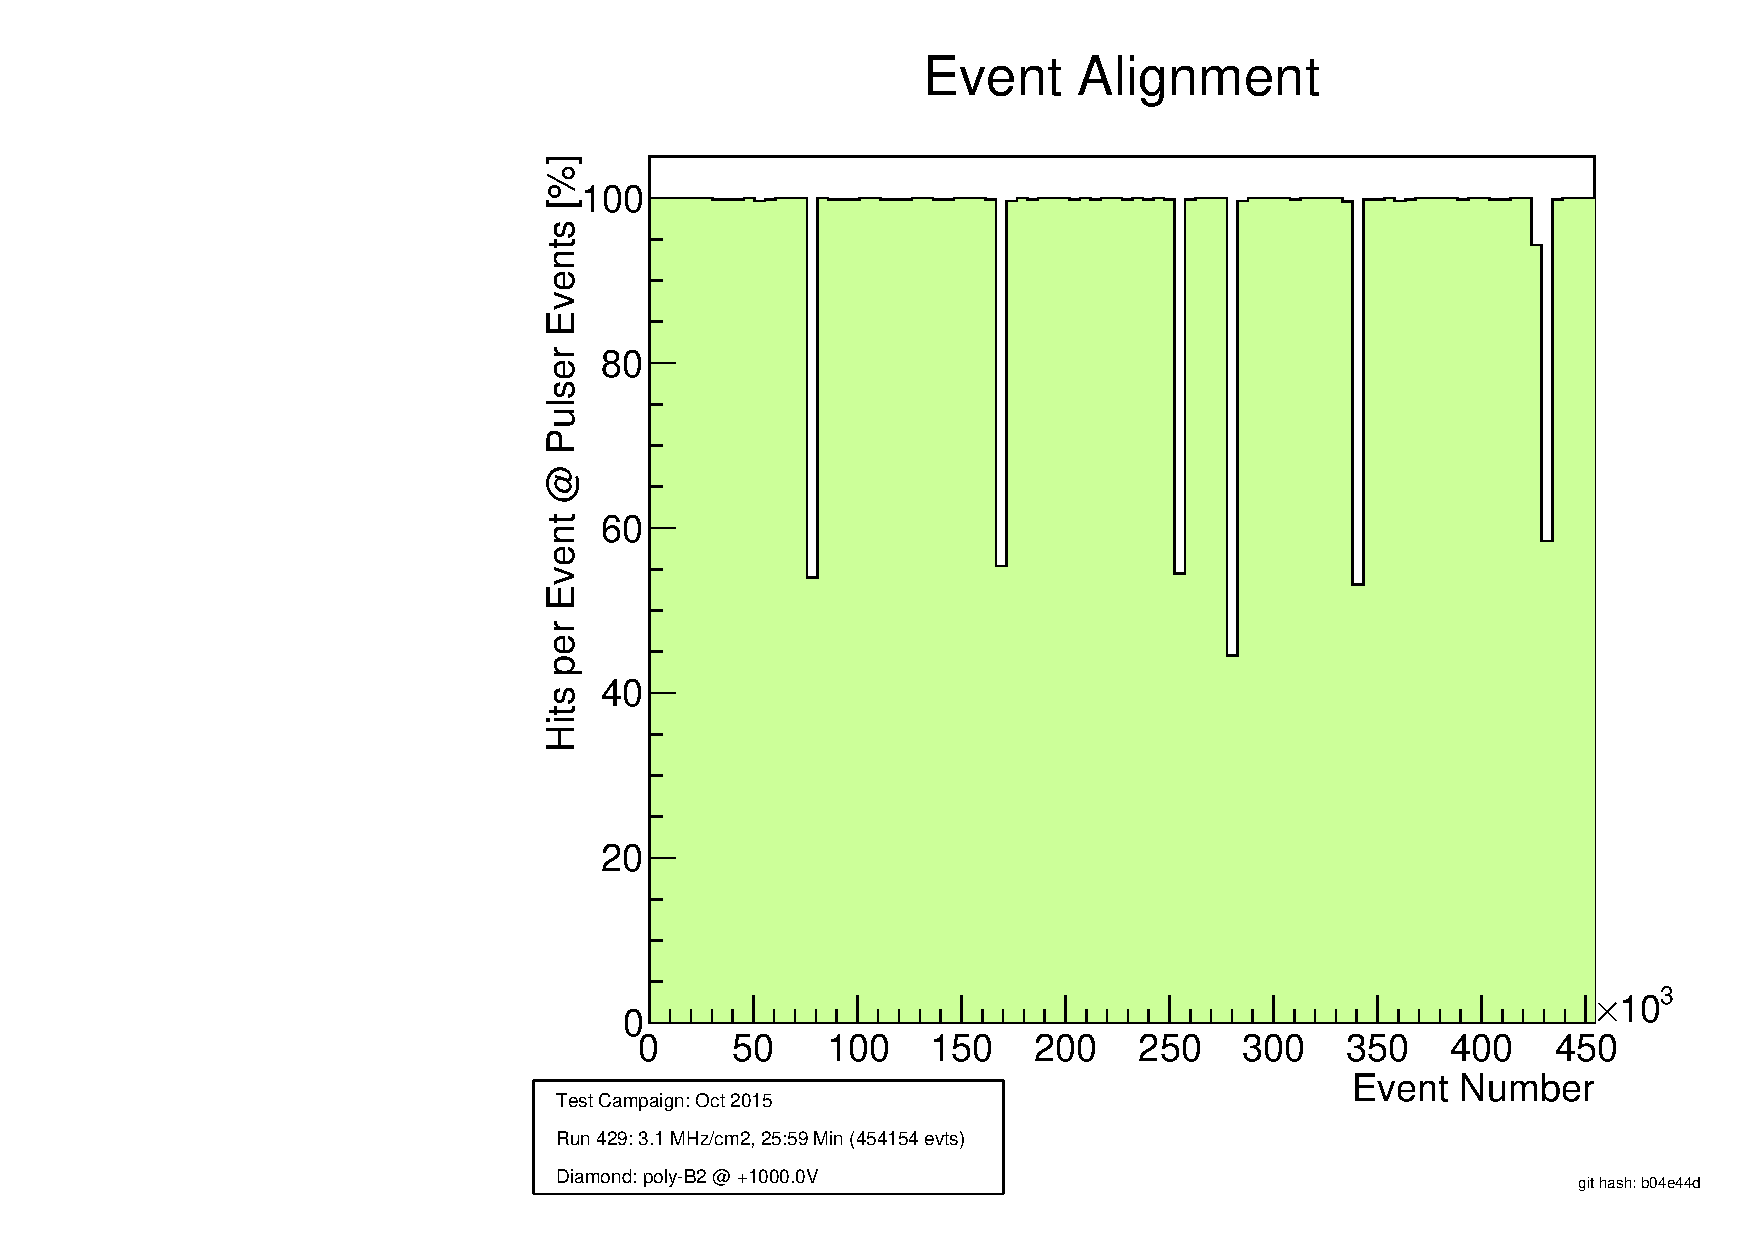
\includegraphics[angle=270, width=5cm]{EventAlignment429}
	\end{center}
	\begin{alertblock}{
		\begin{center}
			\textbf{Event Alignment}
		\end{center}}
		\vspace*{10pt}
		\begin{center}\small
		Speaker: Michael Reichmann
		\end{center}\normalsize
	\end{alertblock}
\end{frame}
% END
% ============================
% BEGIN TABLE OF CONTENTS
% ============================
\begin{frame}[allowframebreaks]
	\frametitle{Table of contents}
	\tableofcontents   % [pausesections]
\end{frame}
% END
% ====================================================================================
% BEGIN INTRO
% ====================================================================================
\section{Introduction}
% ============================
\begin{frame}
	\frametitle{Introduction}
	\begin{minipage}[c][.5\textheight]{\textwidth}
		\begin{itemize}
			\setlength{\itemsep}{\fill}
			\item event based data taking
			\item possibility to get event misalignment between diamond and telescope data
			\item all telescope cuts would be meaningless
			\item exclusion of many good events
			\item flat diamond signal map
		\end{itemize}
	\end{minipage}
\end{frame}
% ====================================================================================
% BEGIN EVENT ALIGNMENT
% ====================================================================================
\section{Event Alignment}
% ============================
\subsection{Aligning}
\begin{frame}
	\begin{minipage}{5.5cm}
		\centering
		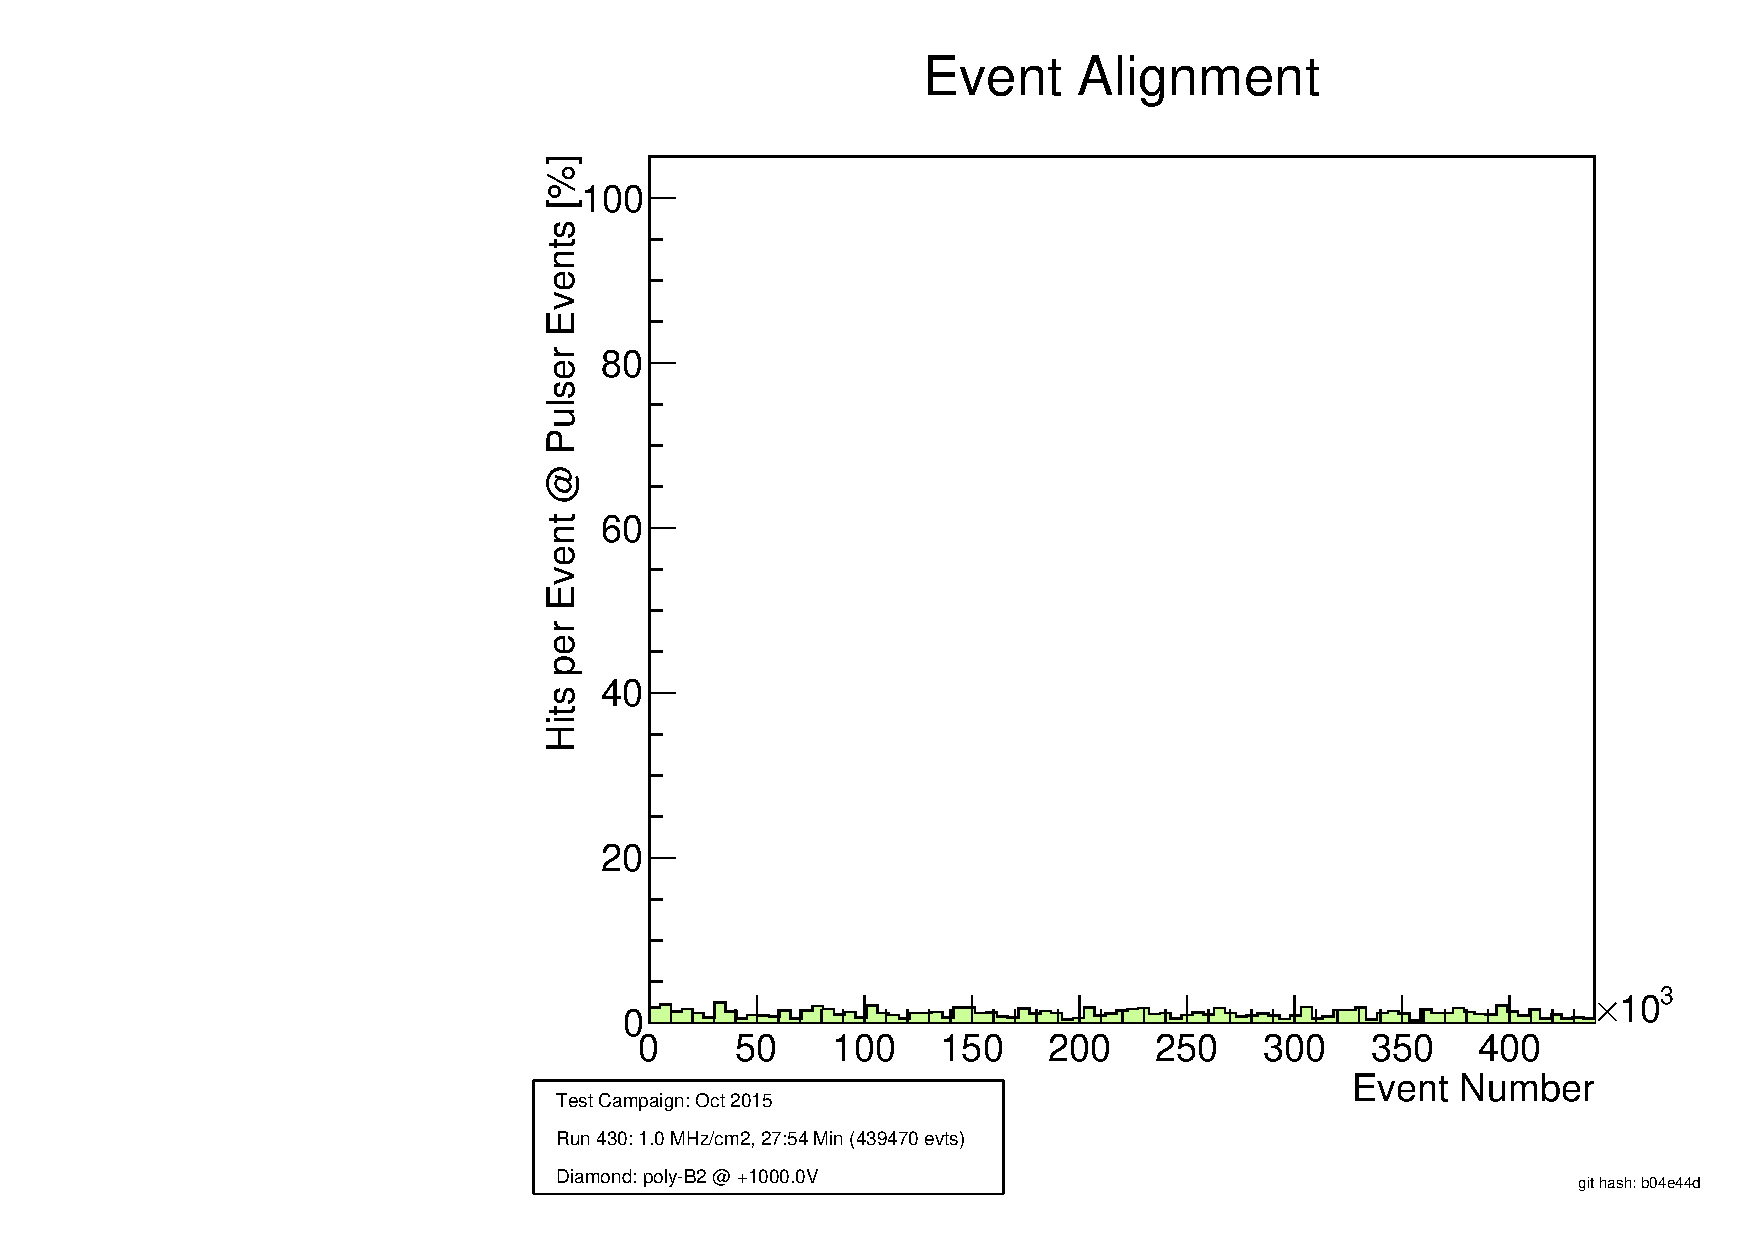
\includegraphics[angle=270, width=5.5cm]{EventAlignment430}
	\end{minipage}
	\hspace*{2pt}
	\begin{minipage}{5.5cm}
		\centering
		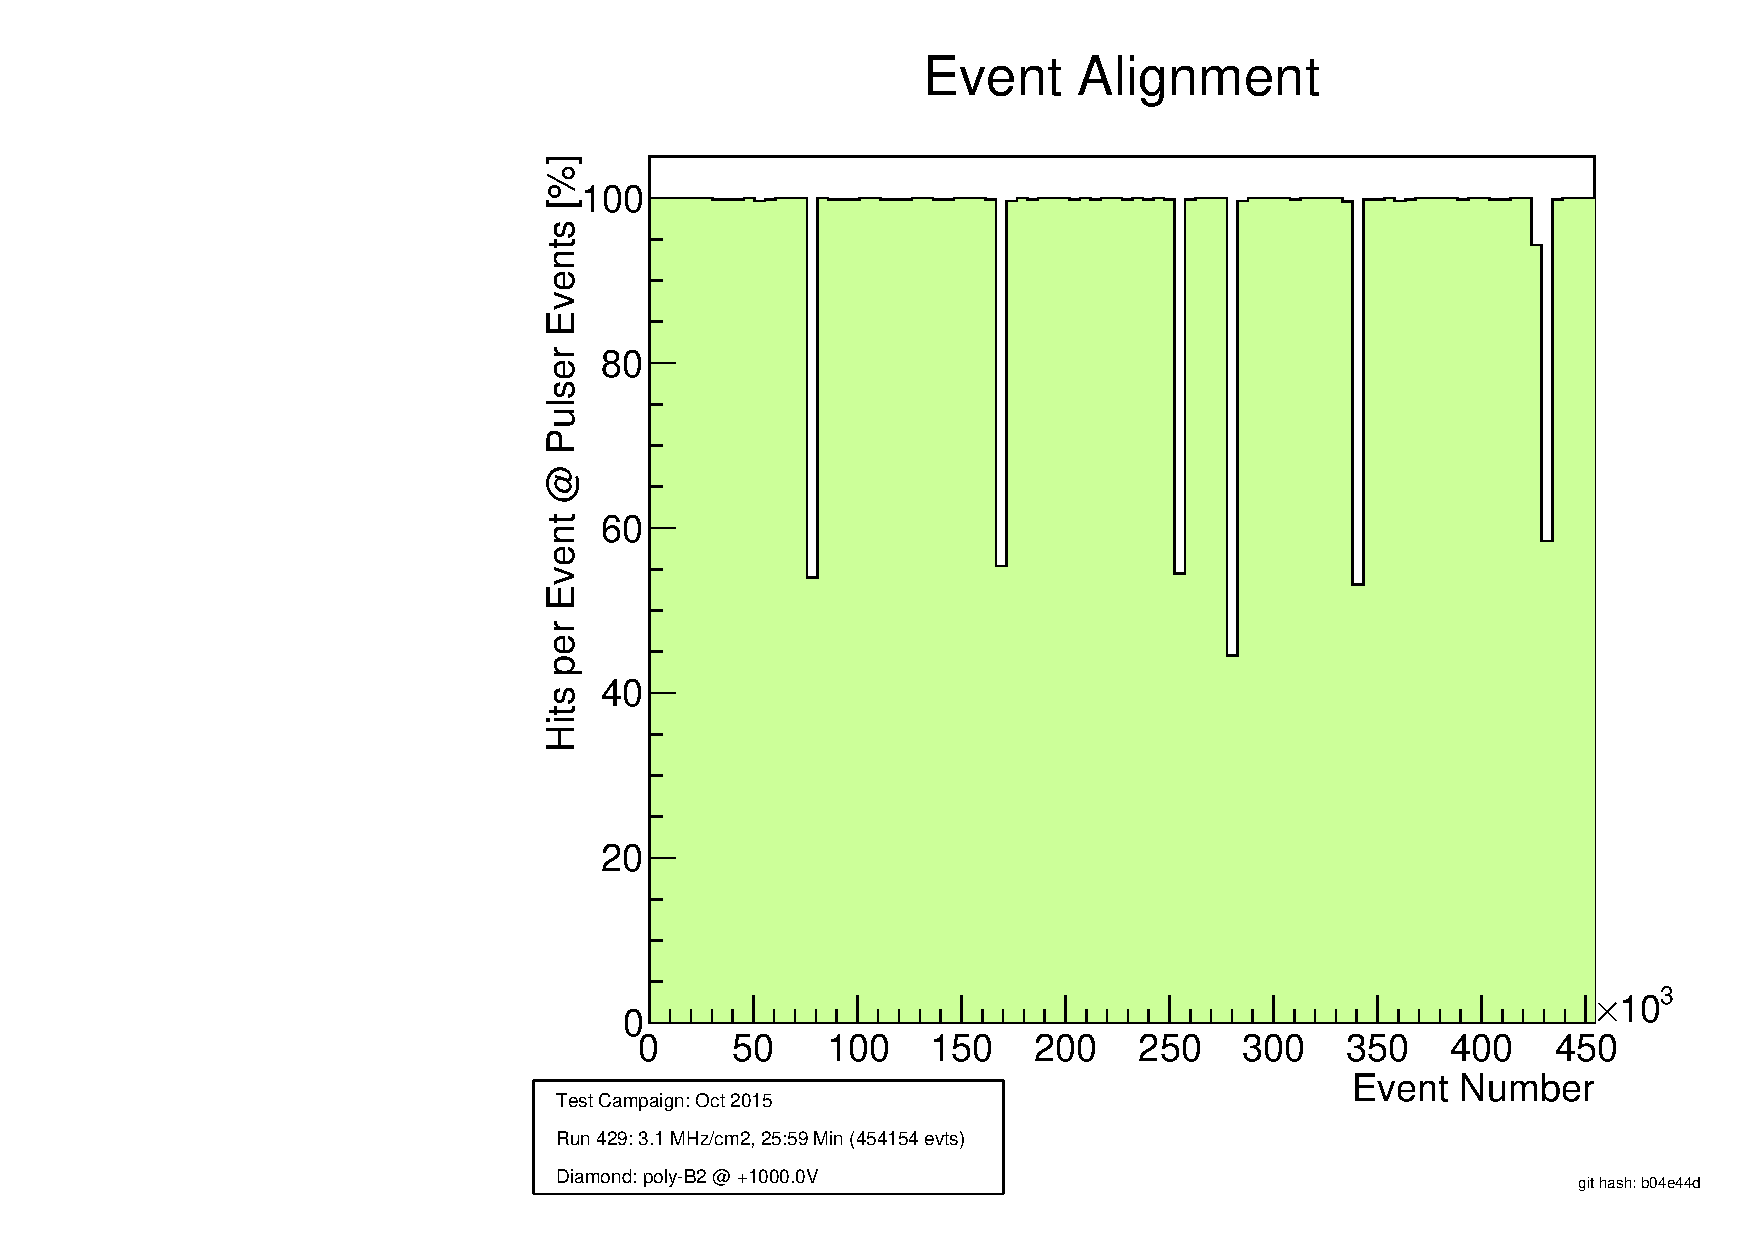
\includegraphics[angle=270, width=5.5cm]{EventAlignment429}
	\end{minipage}\s
	\begin{itemize}
		\item check if there is a hit in any plane at the pulser events of the DRS4
		\item we only have pulser events at if there was no trigger from the telescope
		\begin{itemize}
			\item expect only random hits at these pulser events
		\end{itemize}
		\item very good indicator for misalignment of DTB and DRS4
	\end{itemize}
\end{frame}
% new frame ============================
\begin{frame}
	\begin{center}
		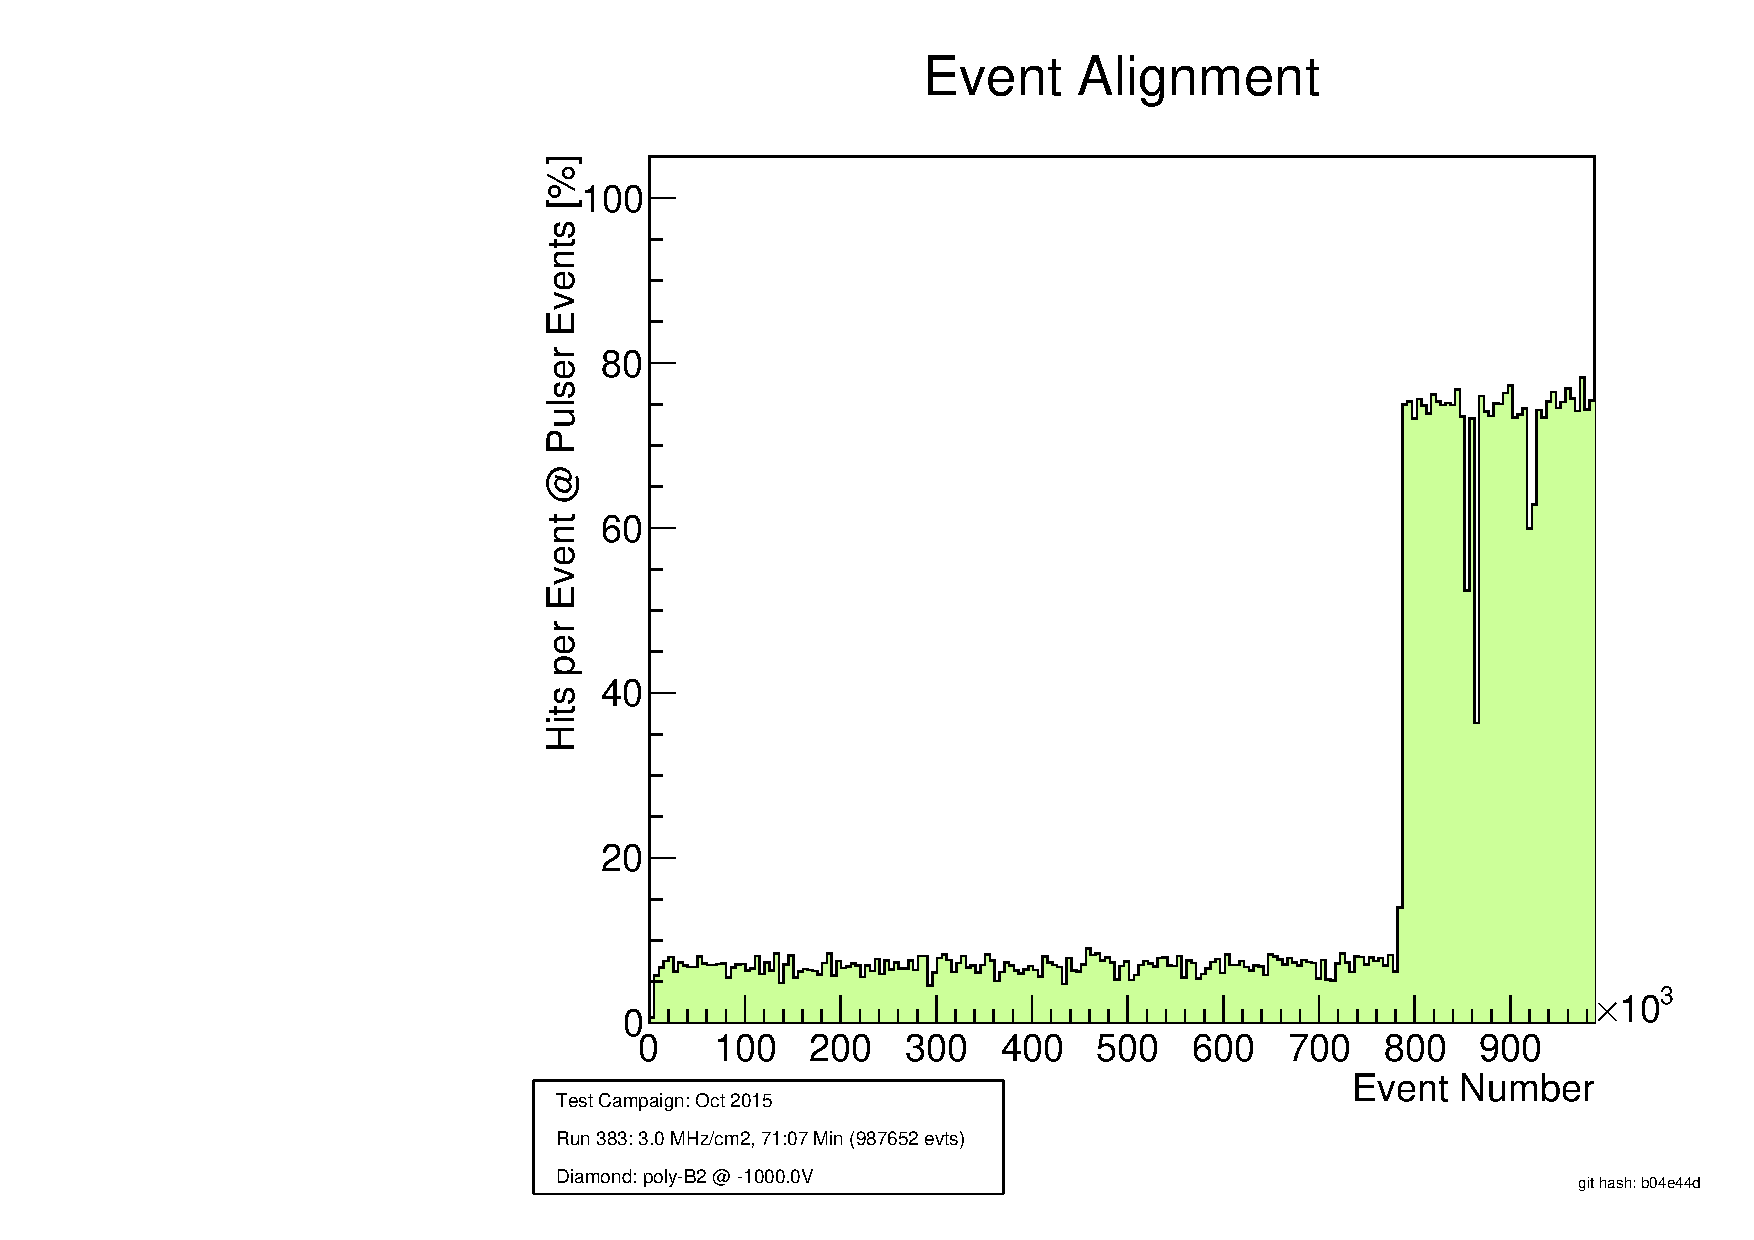
\includegraphics[angle=270, width=5.5cm]{EventAlignment383}
	\end{center}
	\begin{itemize}
		\item usually event misalignment right from the start:
		\begin{itemize}
			\item offset is $-1$ which means that the DRS4 is 1 event behind
		\end{itemize}
		\item there also runs which pick up an offset during the run
		\begin{itemize}
			\item positive offset: DTB misses trigger!
		\end{itemize}
	\end{itemize}
\end{frame}
% new frame ============================
\begin{frame}
	\begin{center}
		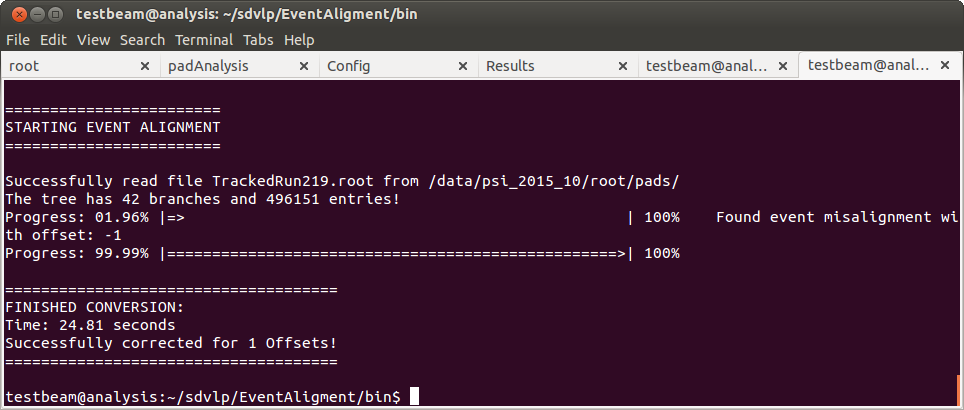
\includegraphics[width=.8\textwidth]{Prog}
	\end{center}
	\begin{itemize}
		\item writing tool in c++ to realign the trees with negative offset
		\item save <N> last events of the telescope branches
		\item check the number of hits for the <N> last telescope events for every <X> pulser events
		\item offset = lowest hit rate 
		\item save the correct telescope event to the DRS4 events by choosing form the last <N>
		\item may correct for a large number of offsets
	\end{itemize}
\end{frame}
% new frame ============================
\begin{frame}
	\begin{minipage}{5.5cm}
		\centering
		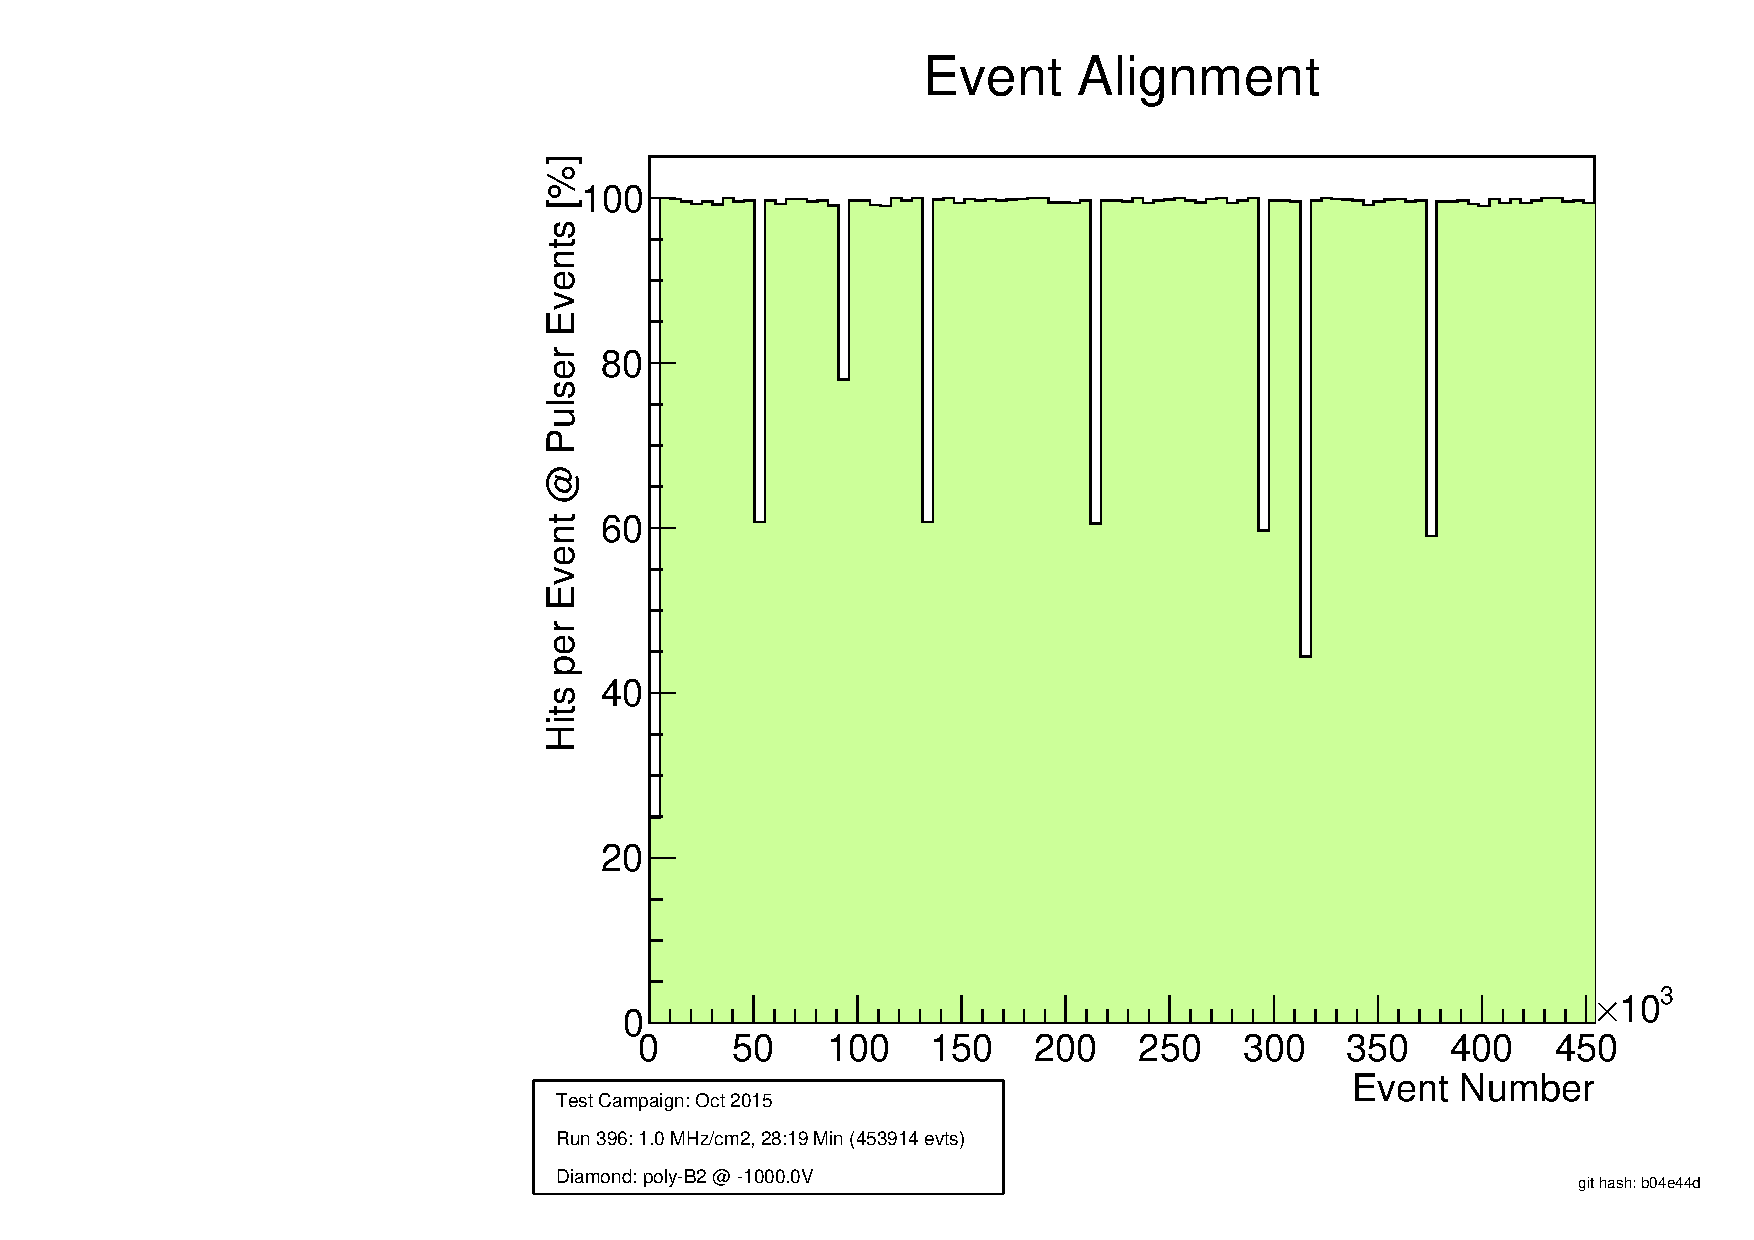
\includegraphics[angle=270, width=5.5cm]{EventAlignment396}
	\end{minipage}
	\hspace*{2pt}
	\begin{minipage}{5.5cm}
		\centering
		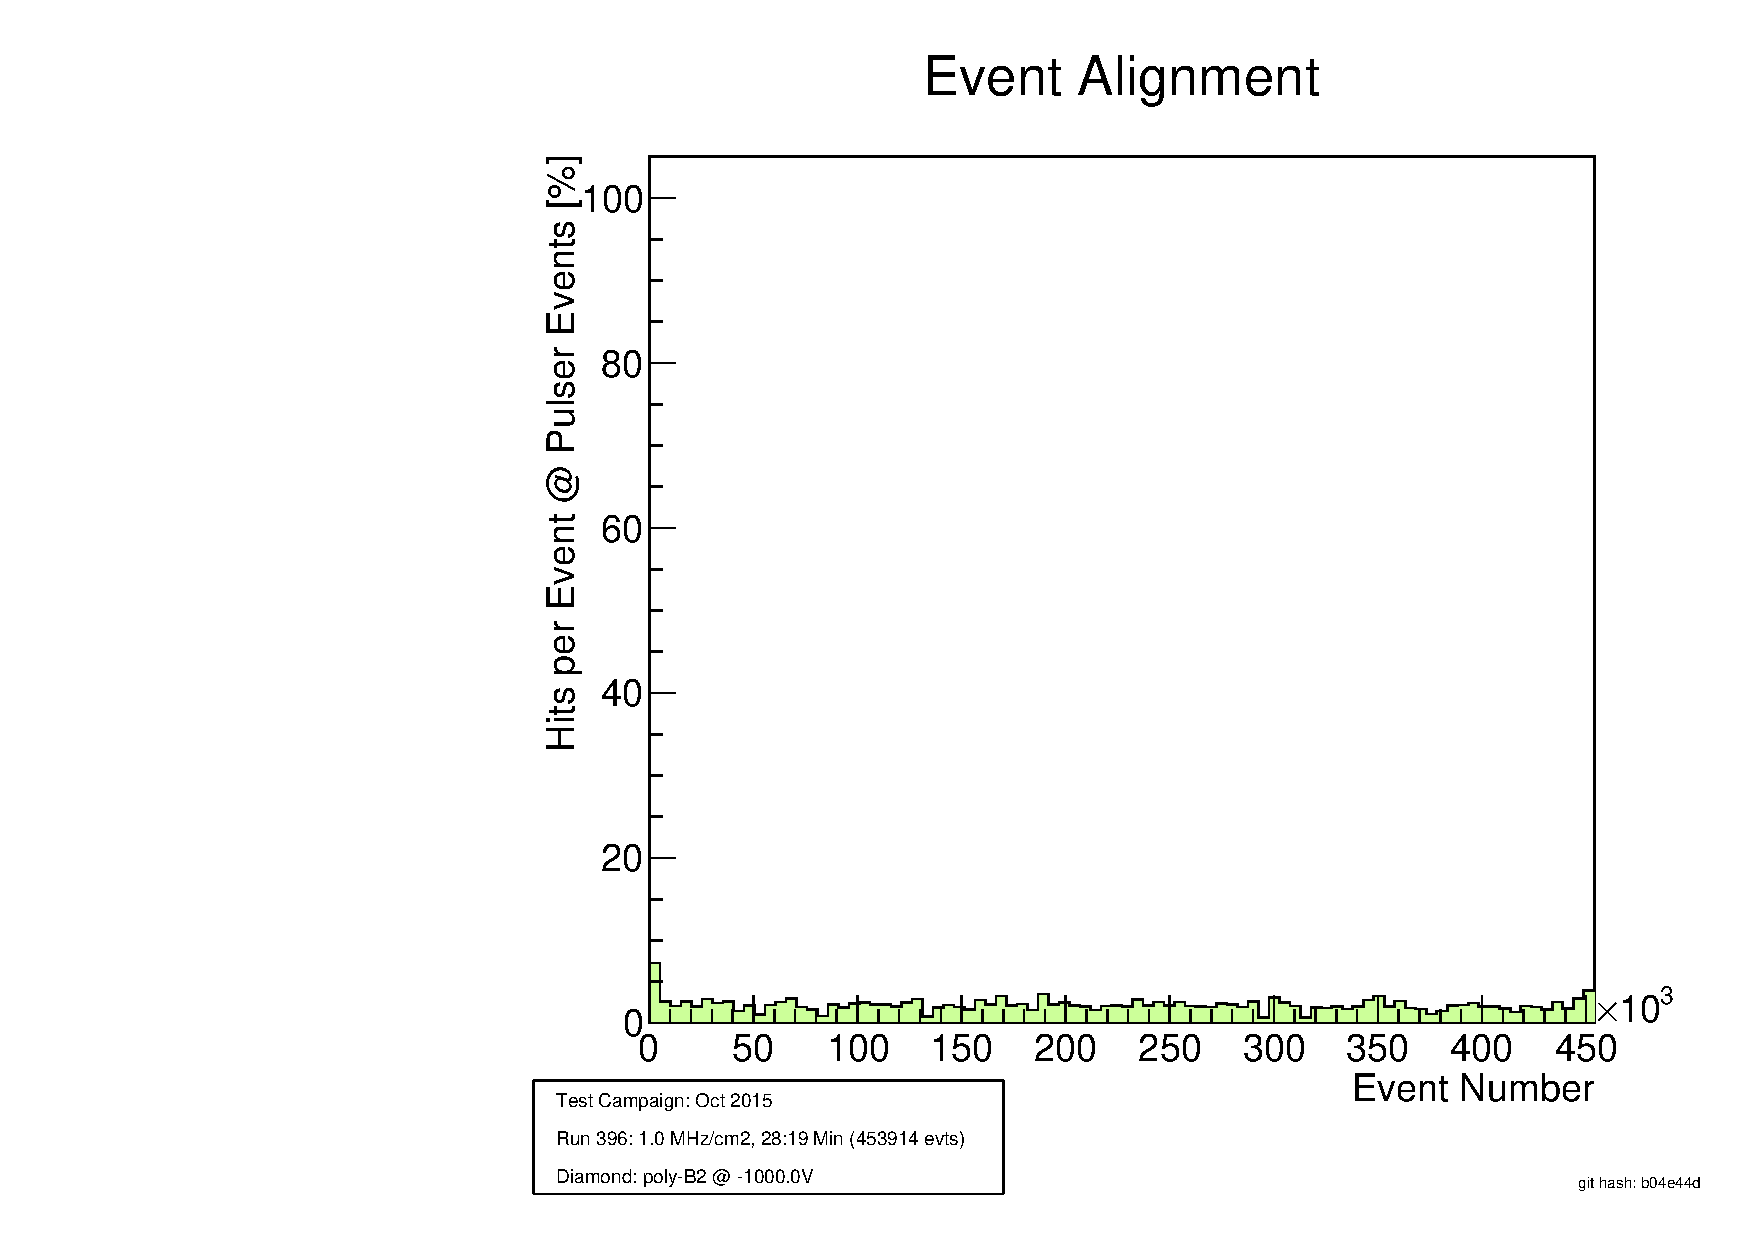
\includegraphics[angle=270, width=5.5cm]{EventAlignment396a}
	\end{minipage}\s
\end{frame}
% new frame ============================
\begin{frame}
	\begin{minipage}{5.5cm}
		\centering
		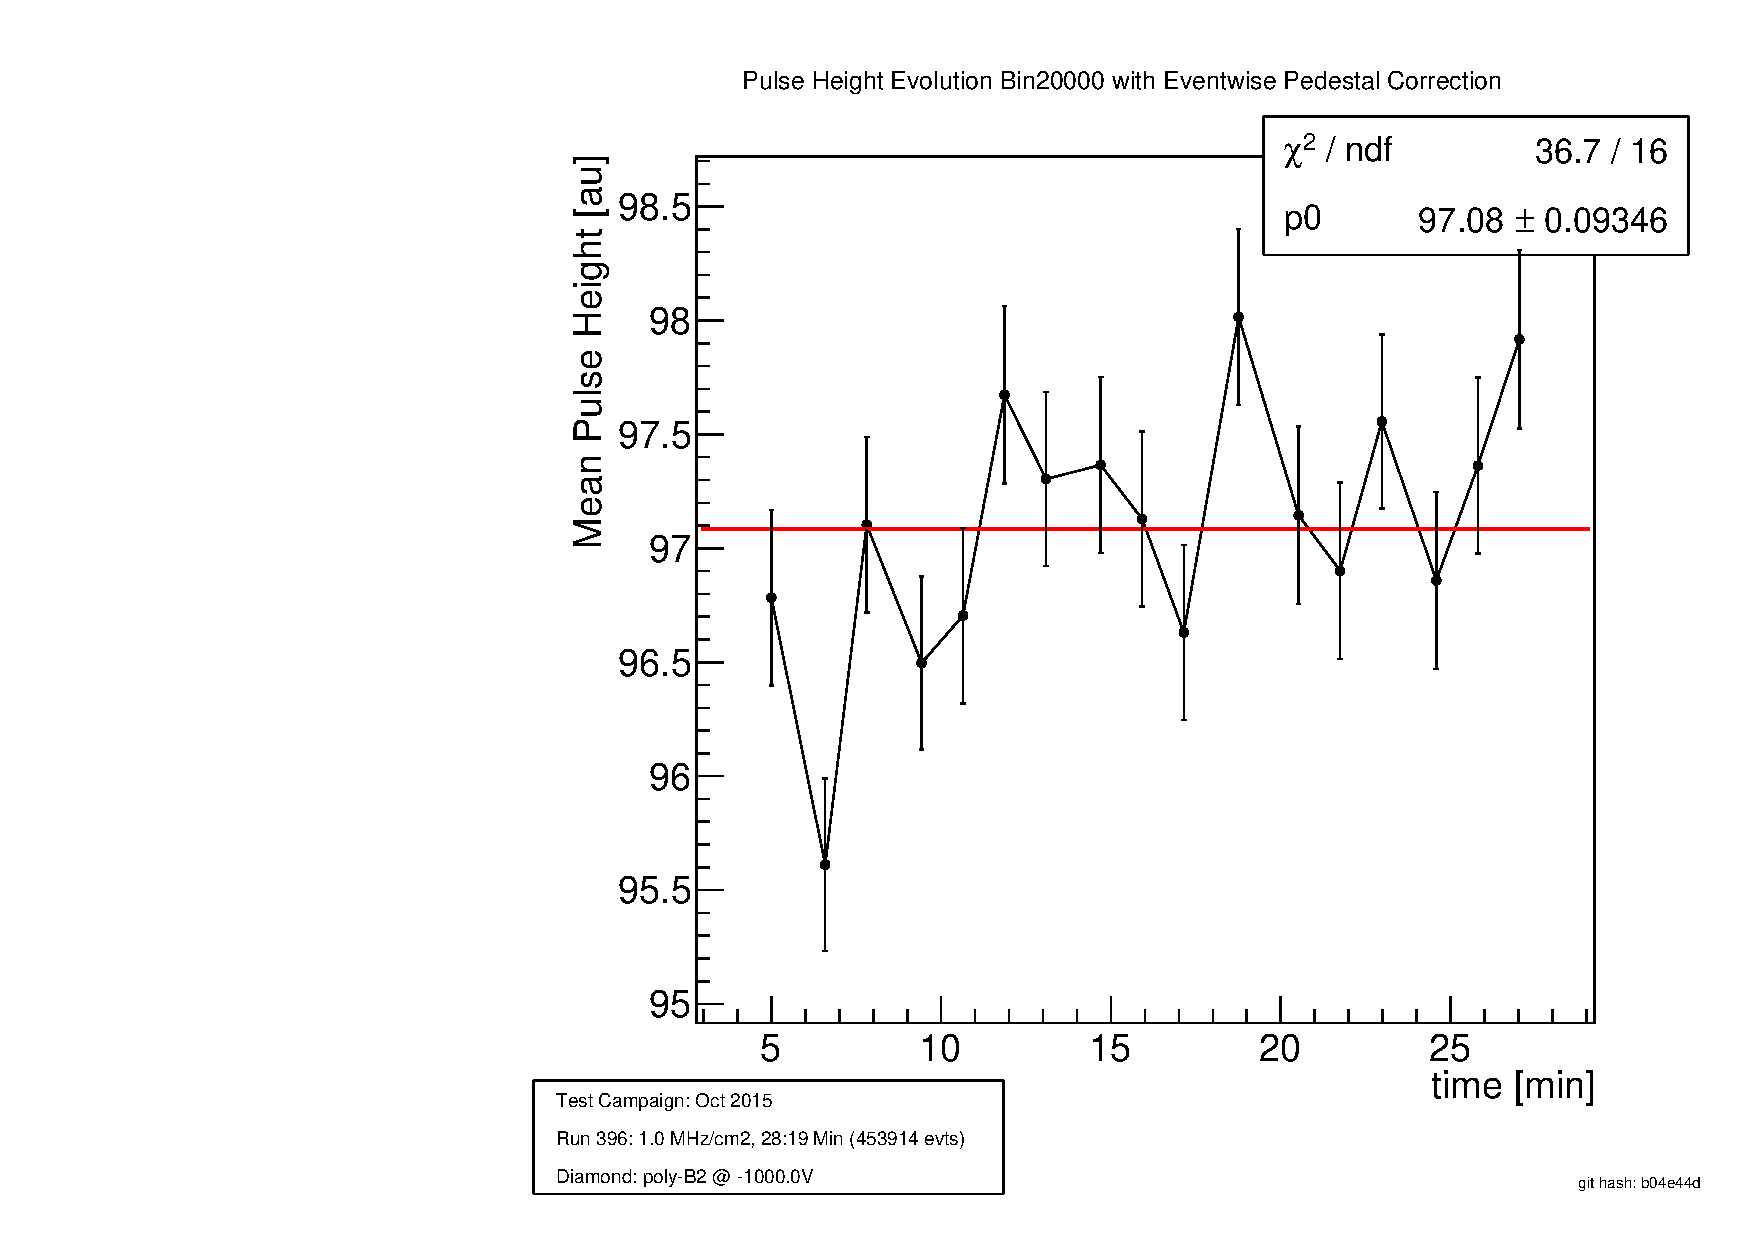
\includegraphics[angle=270, width=5.5cm]{PulseHeight20000396}
	\end{minipage}
	\hspace*{2pt}
	\begin{minipage}{5.5cm}
		\centering
		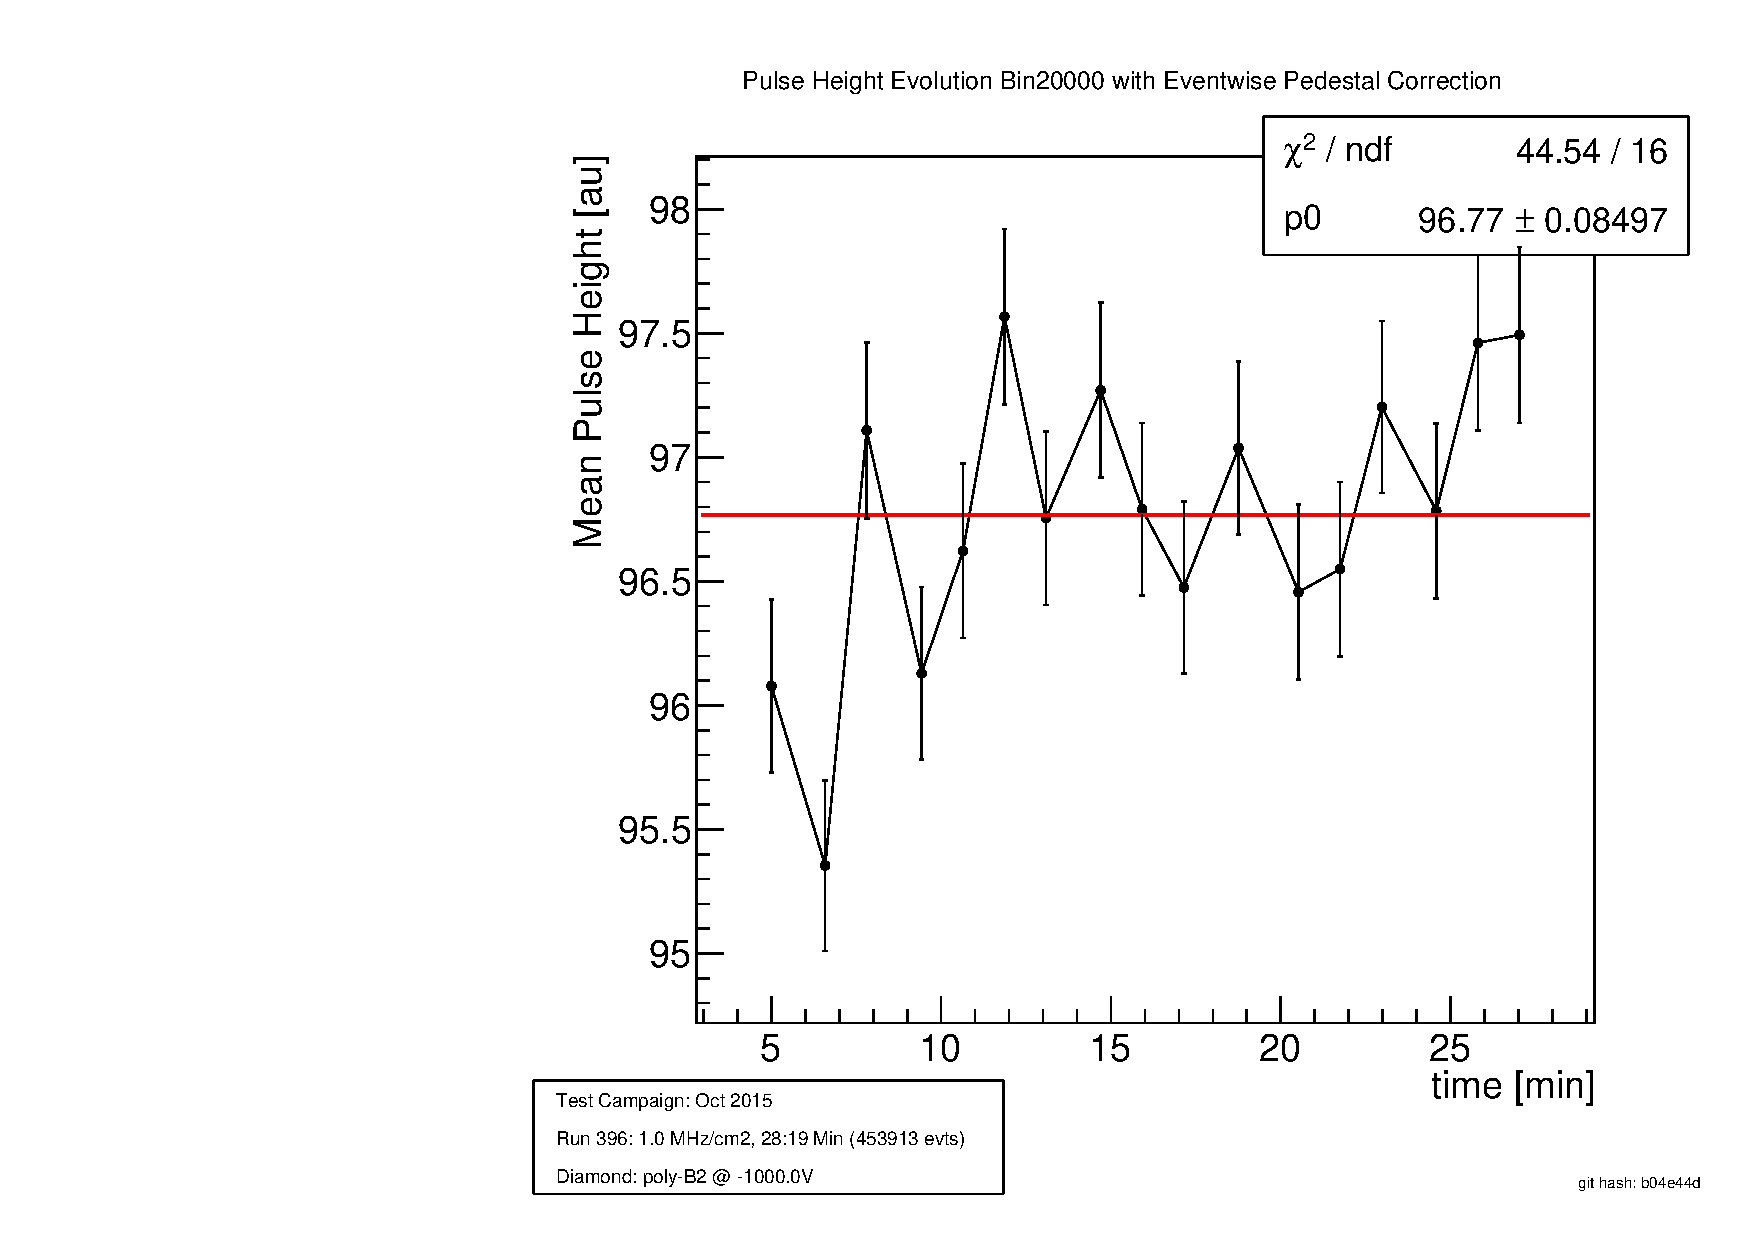
\includegraphics[angle=270, width=5.5cm]{PulseHeight20000396a}
	\end{minipage}\s
\end{frame}
% new frame ============================
\begin{frame}
	\begin{minipage}{5.5cm}
		\centering
		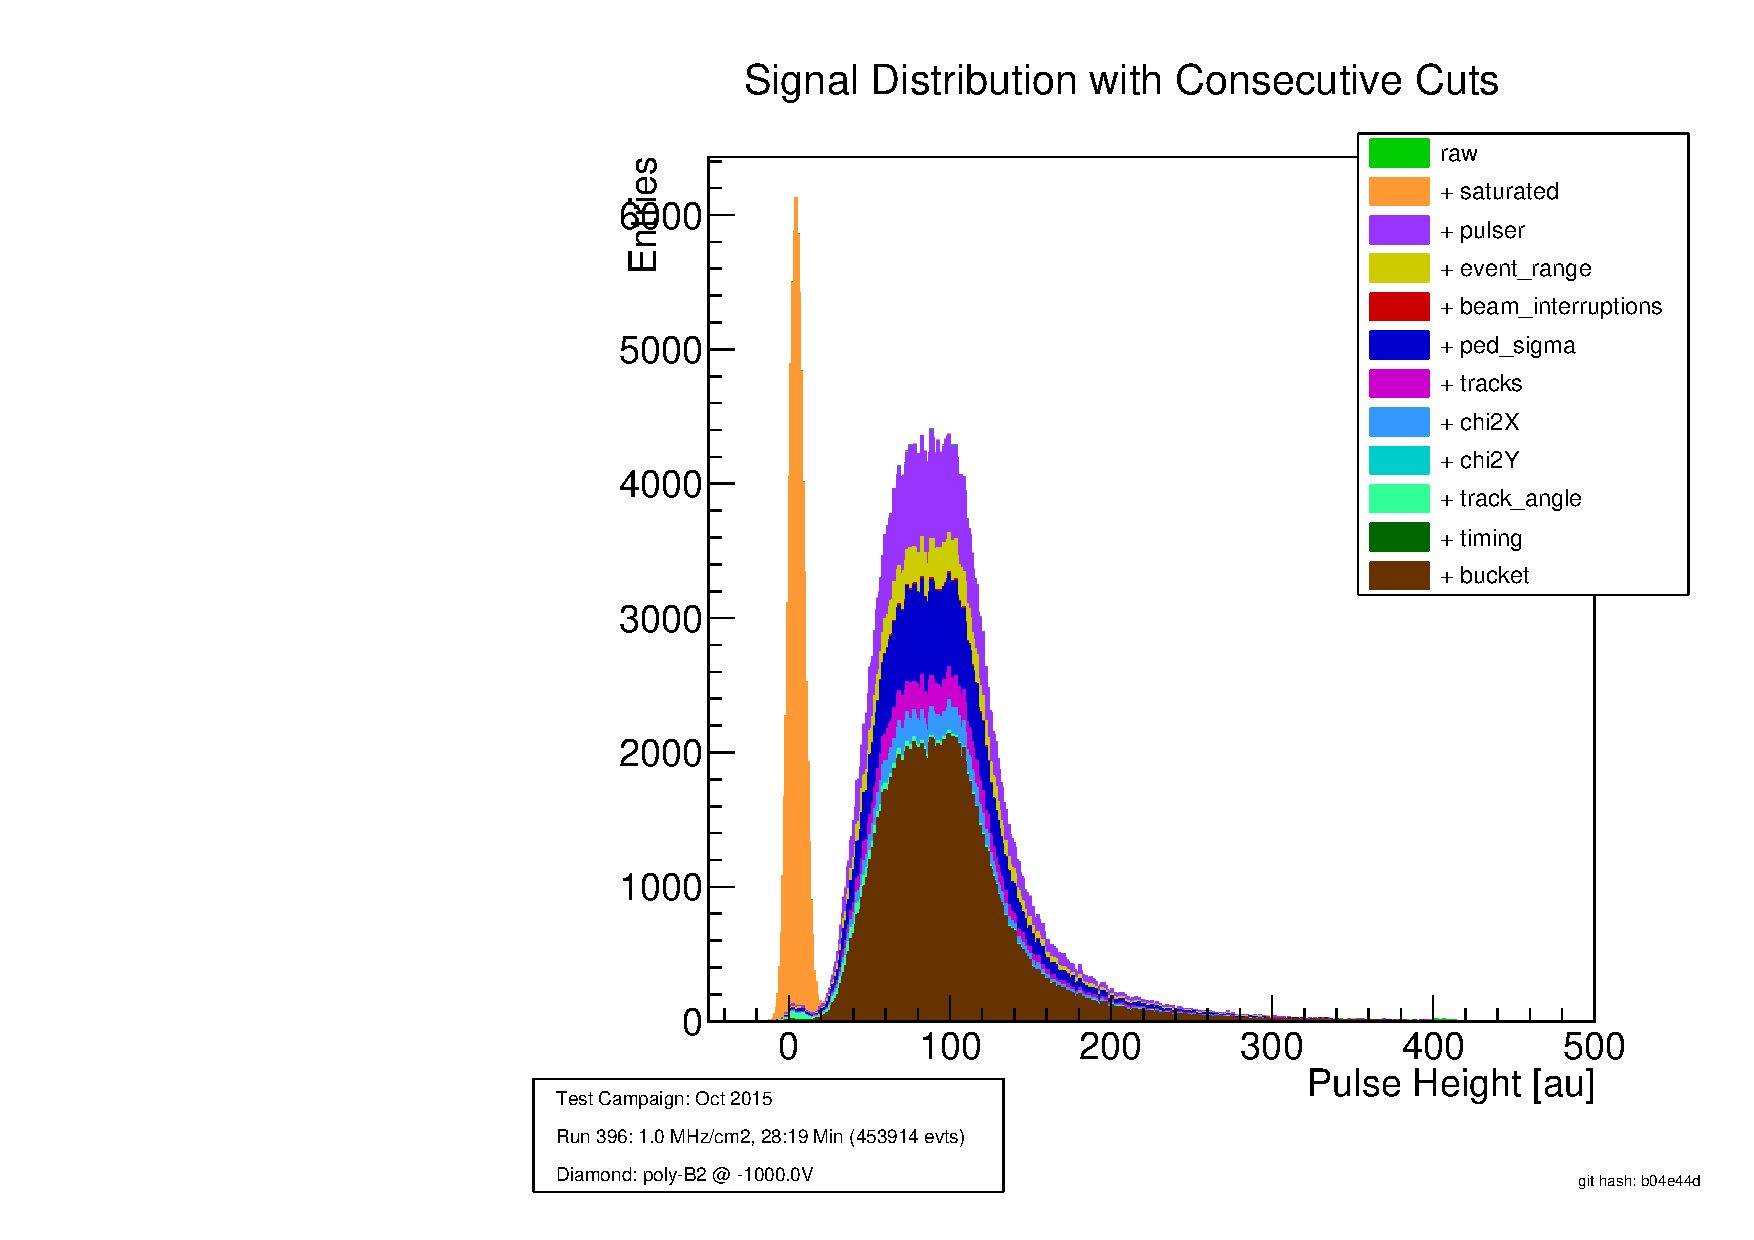
\includegraphics[angle=270, width=4cm]{consecutive396}\\
		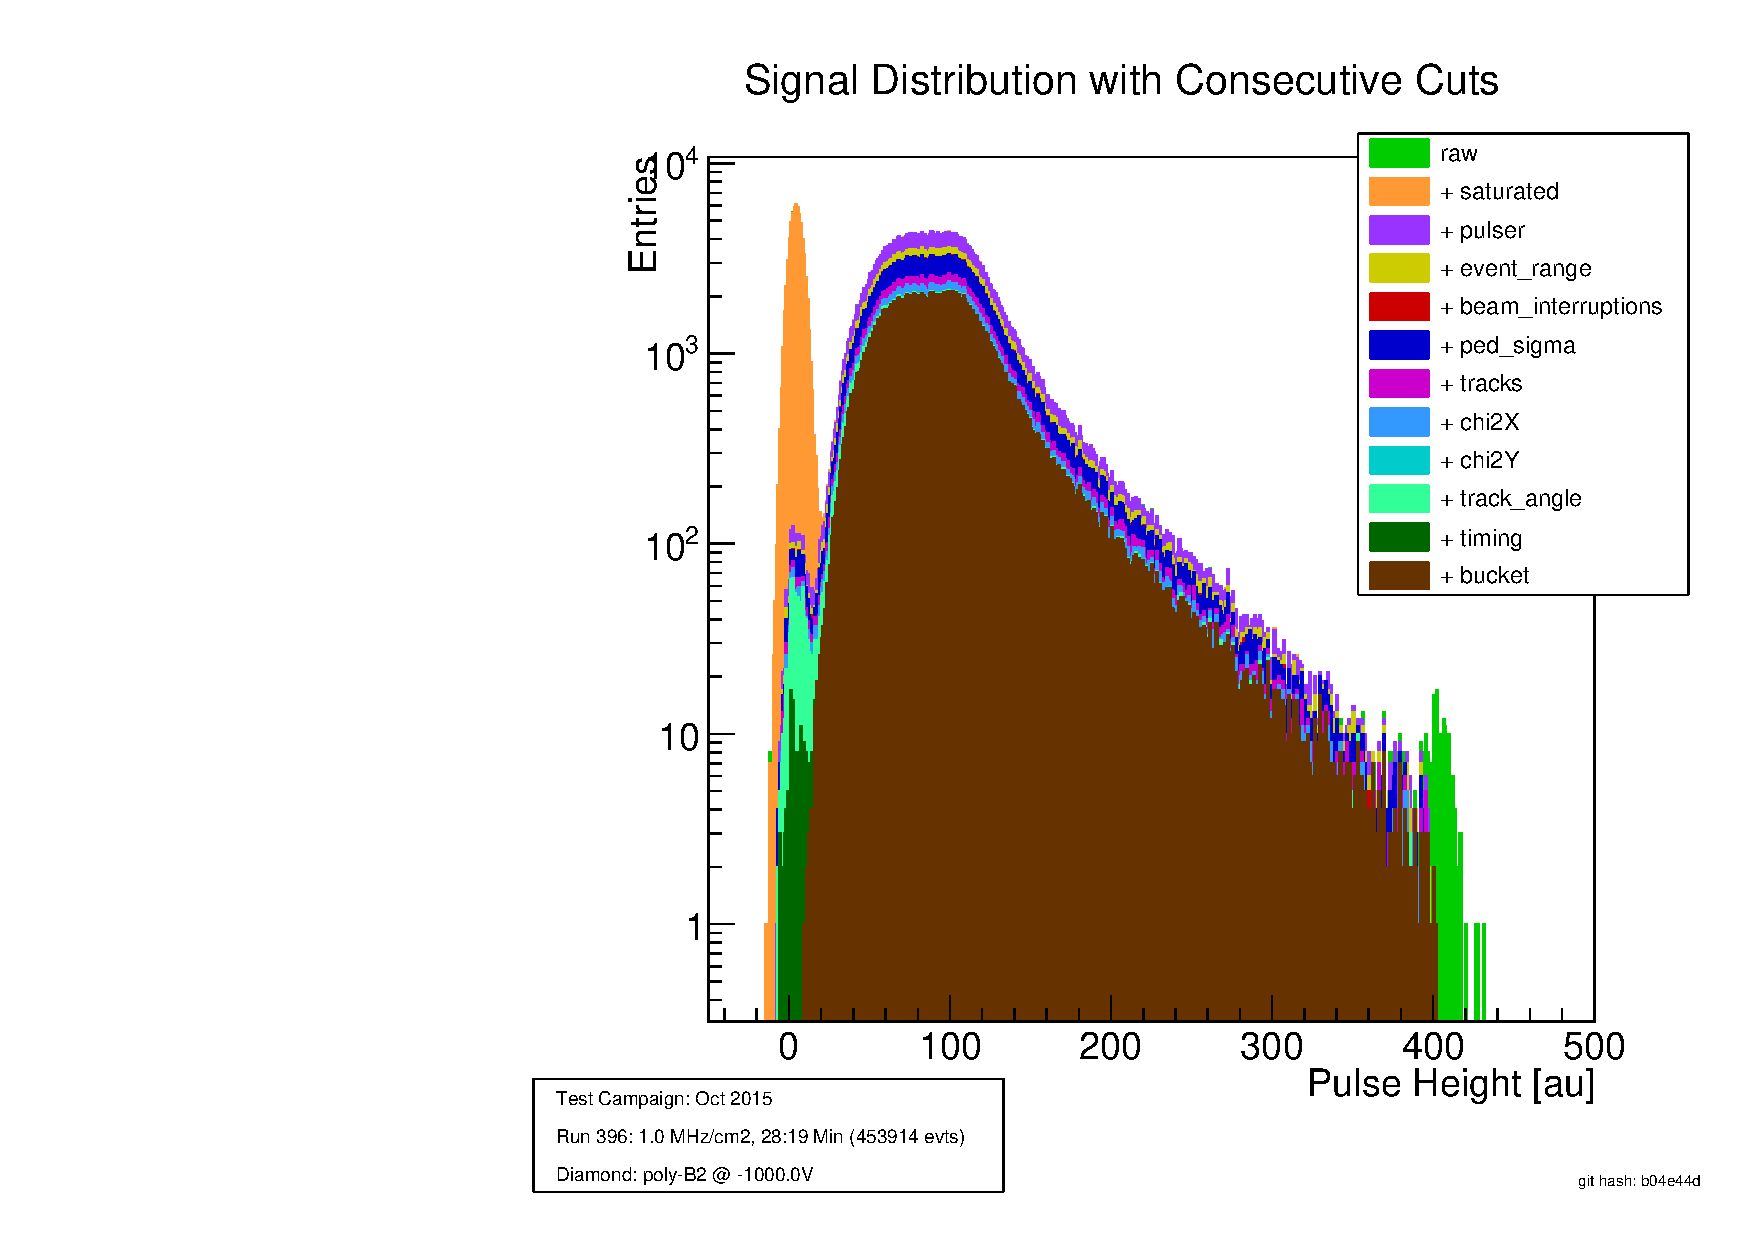
\includegraphics[angle=270, width=4cm]{consecutive_logy396}
	\end{minipage}
	\hspace*{2pt}
	\begin{minipage}{5.5cm}
		\centering
		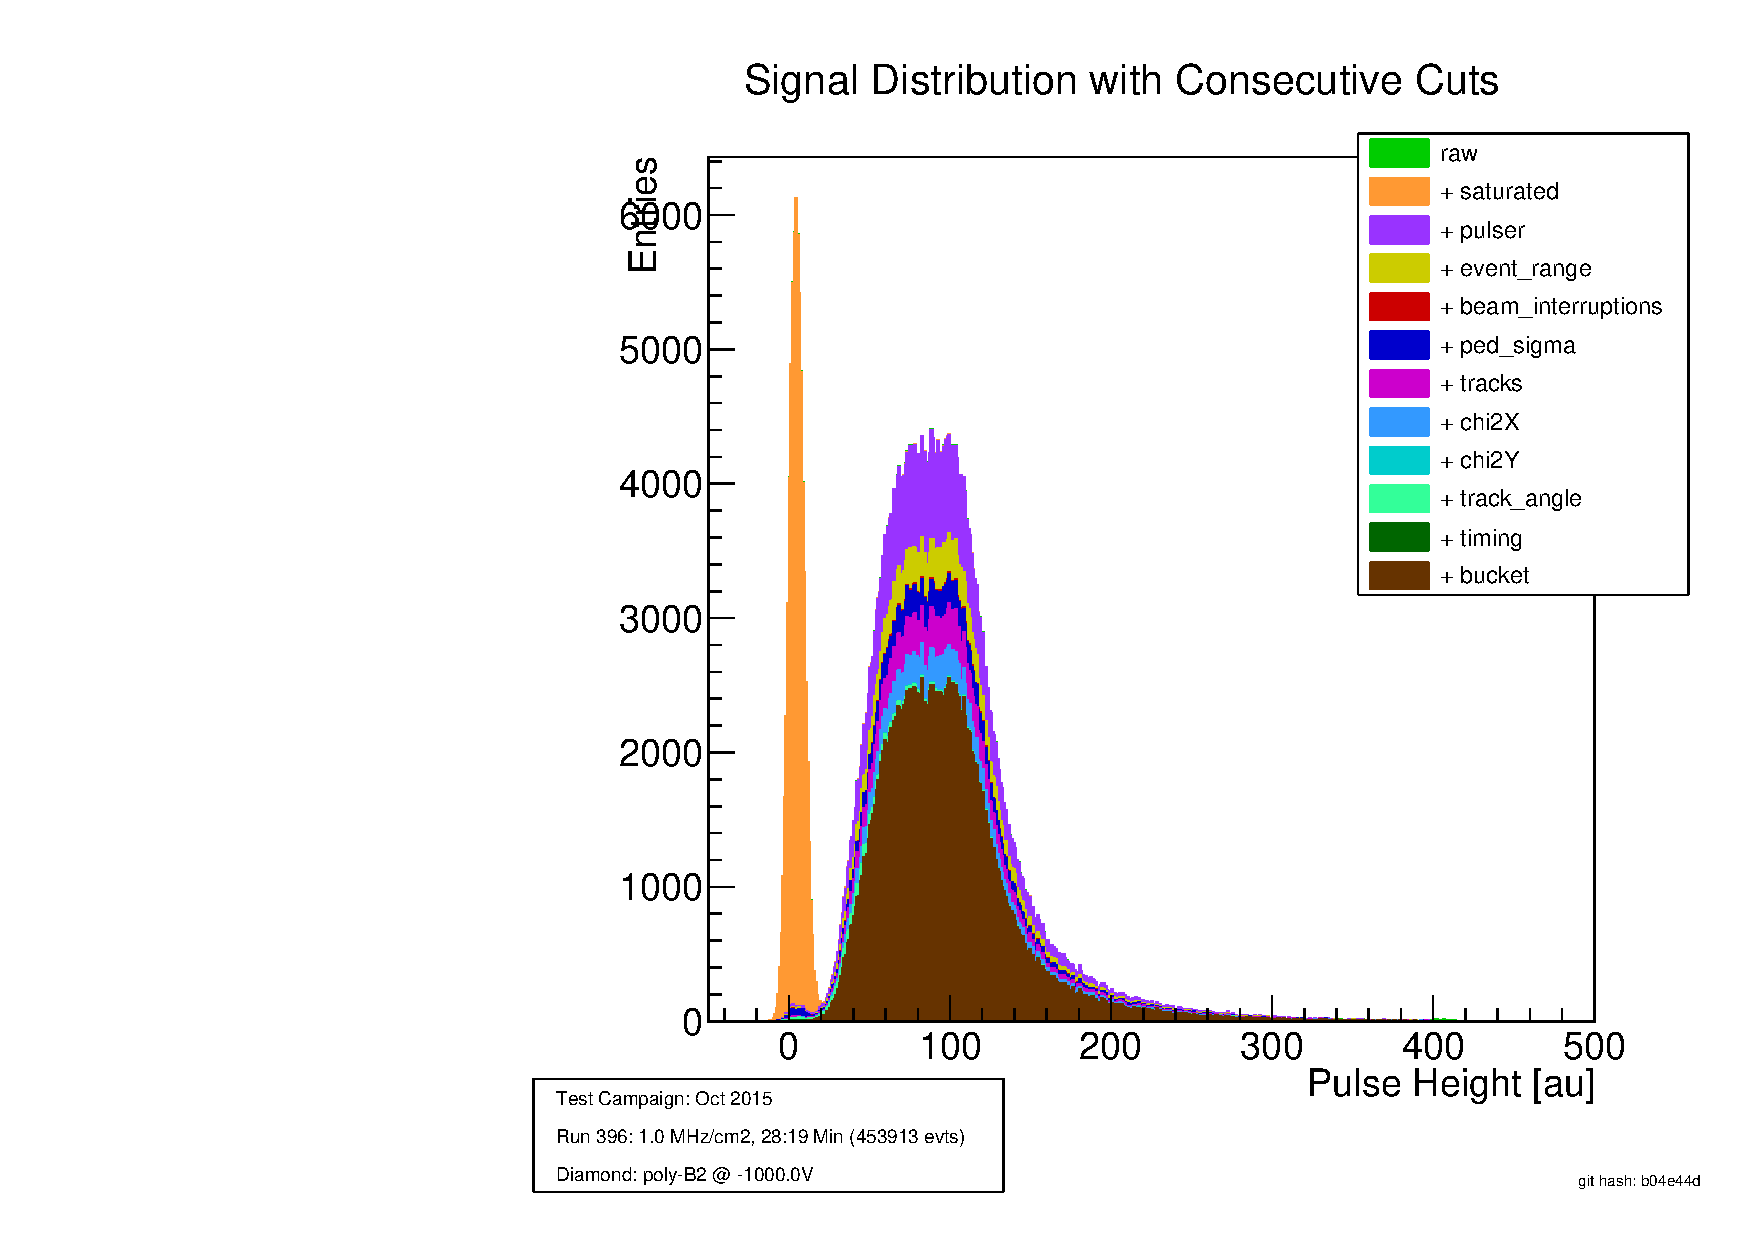
\includegraphics[angle=270, width=4cm]{consecutive396a}\\
		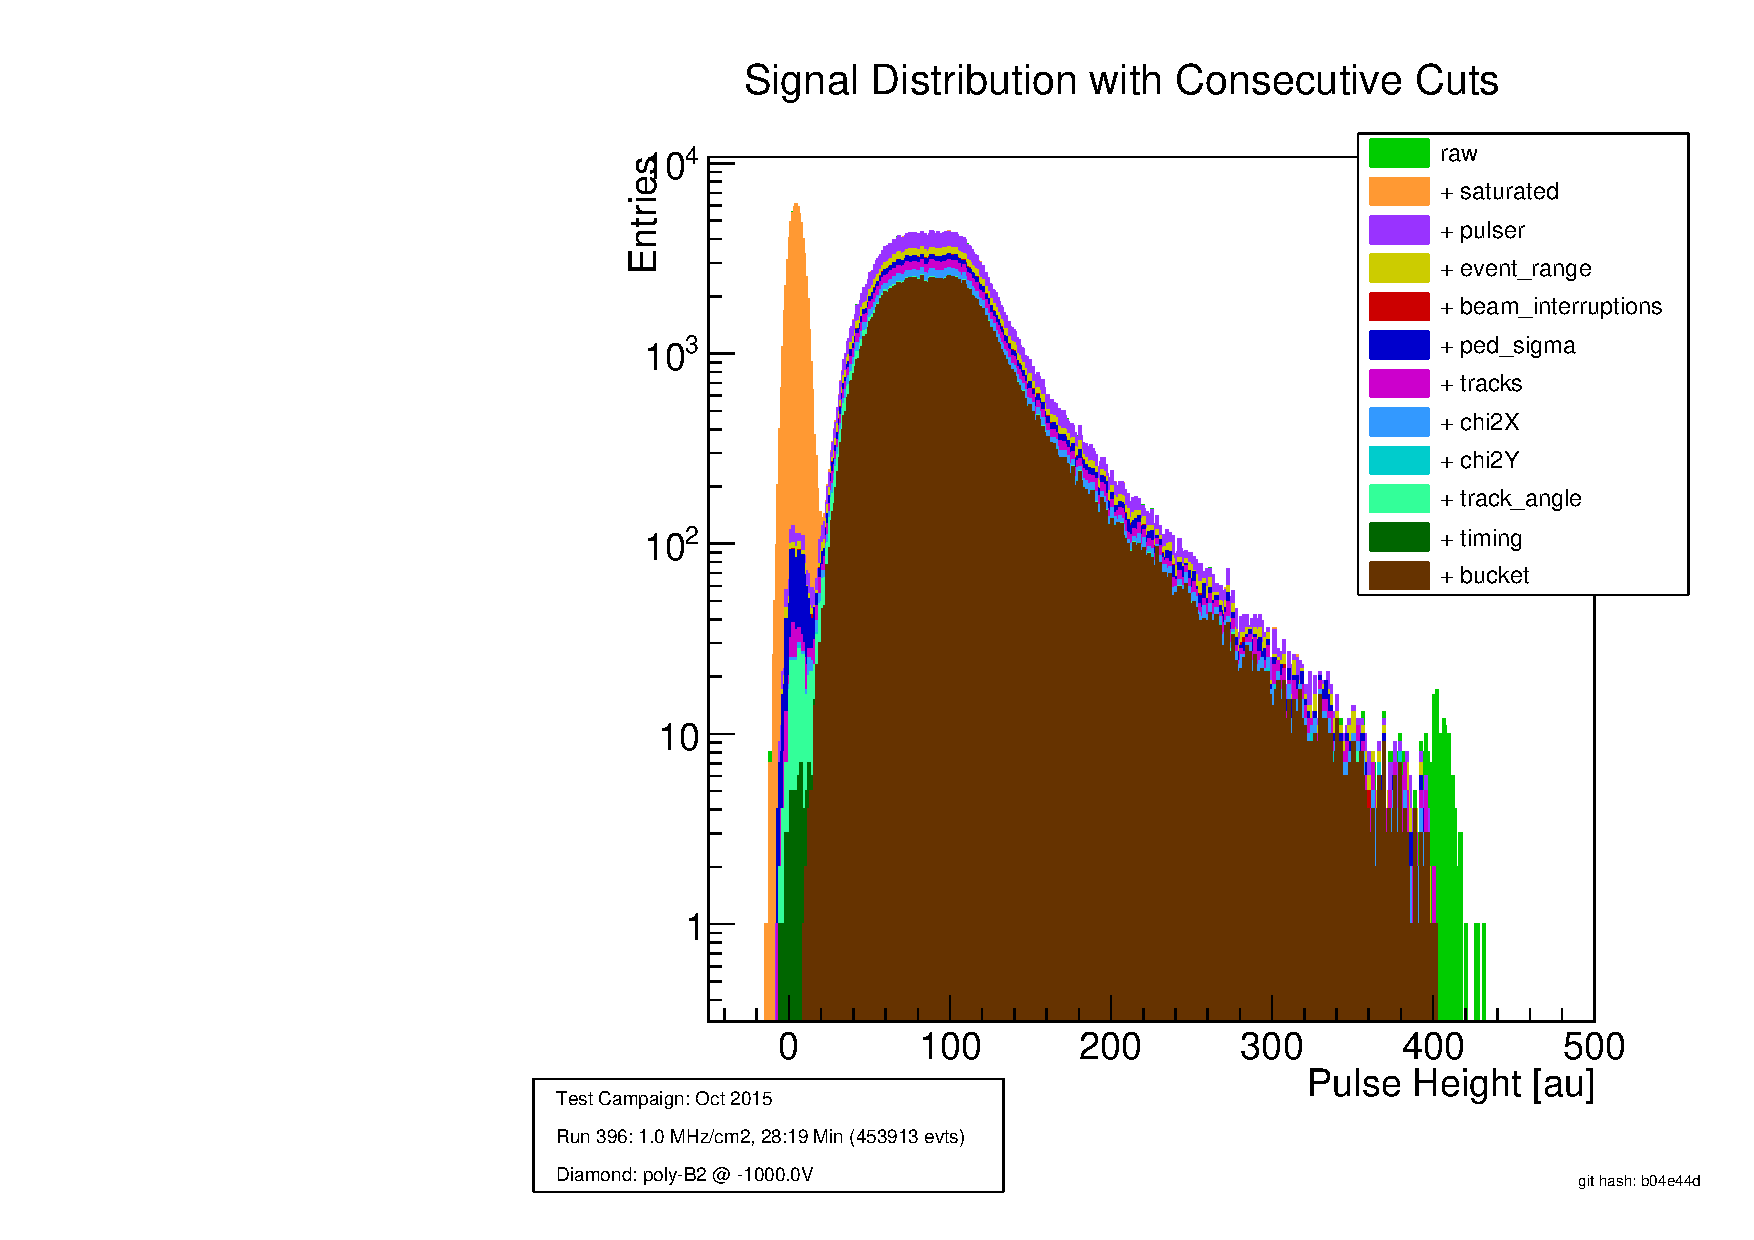
\includegraphics[angle=270, width=4cm]{consecutive_logy396a}
	\end{minipage}\s
\end{frame}
% new frame ============================
\begin{frame}
	\begin{minipage}{5.5cm}
		\centering
		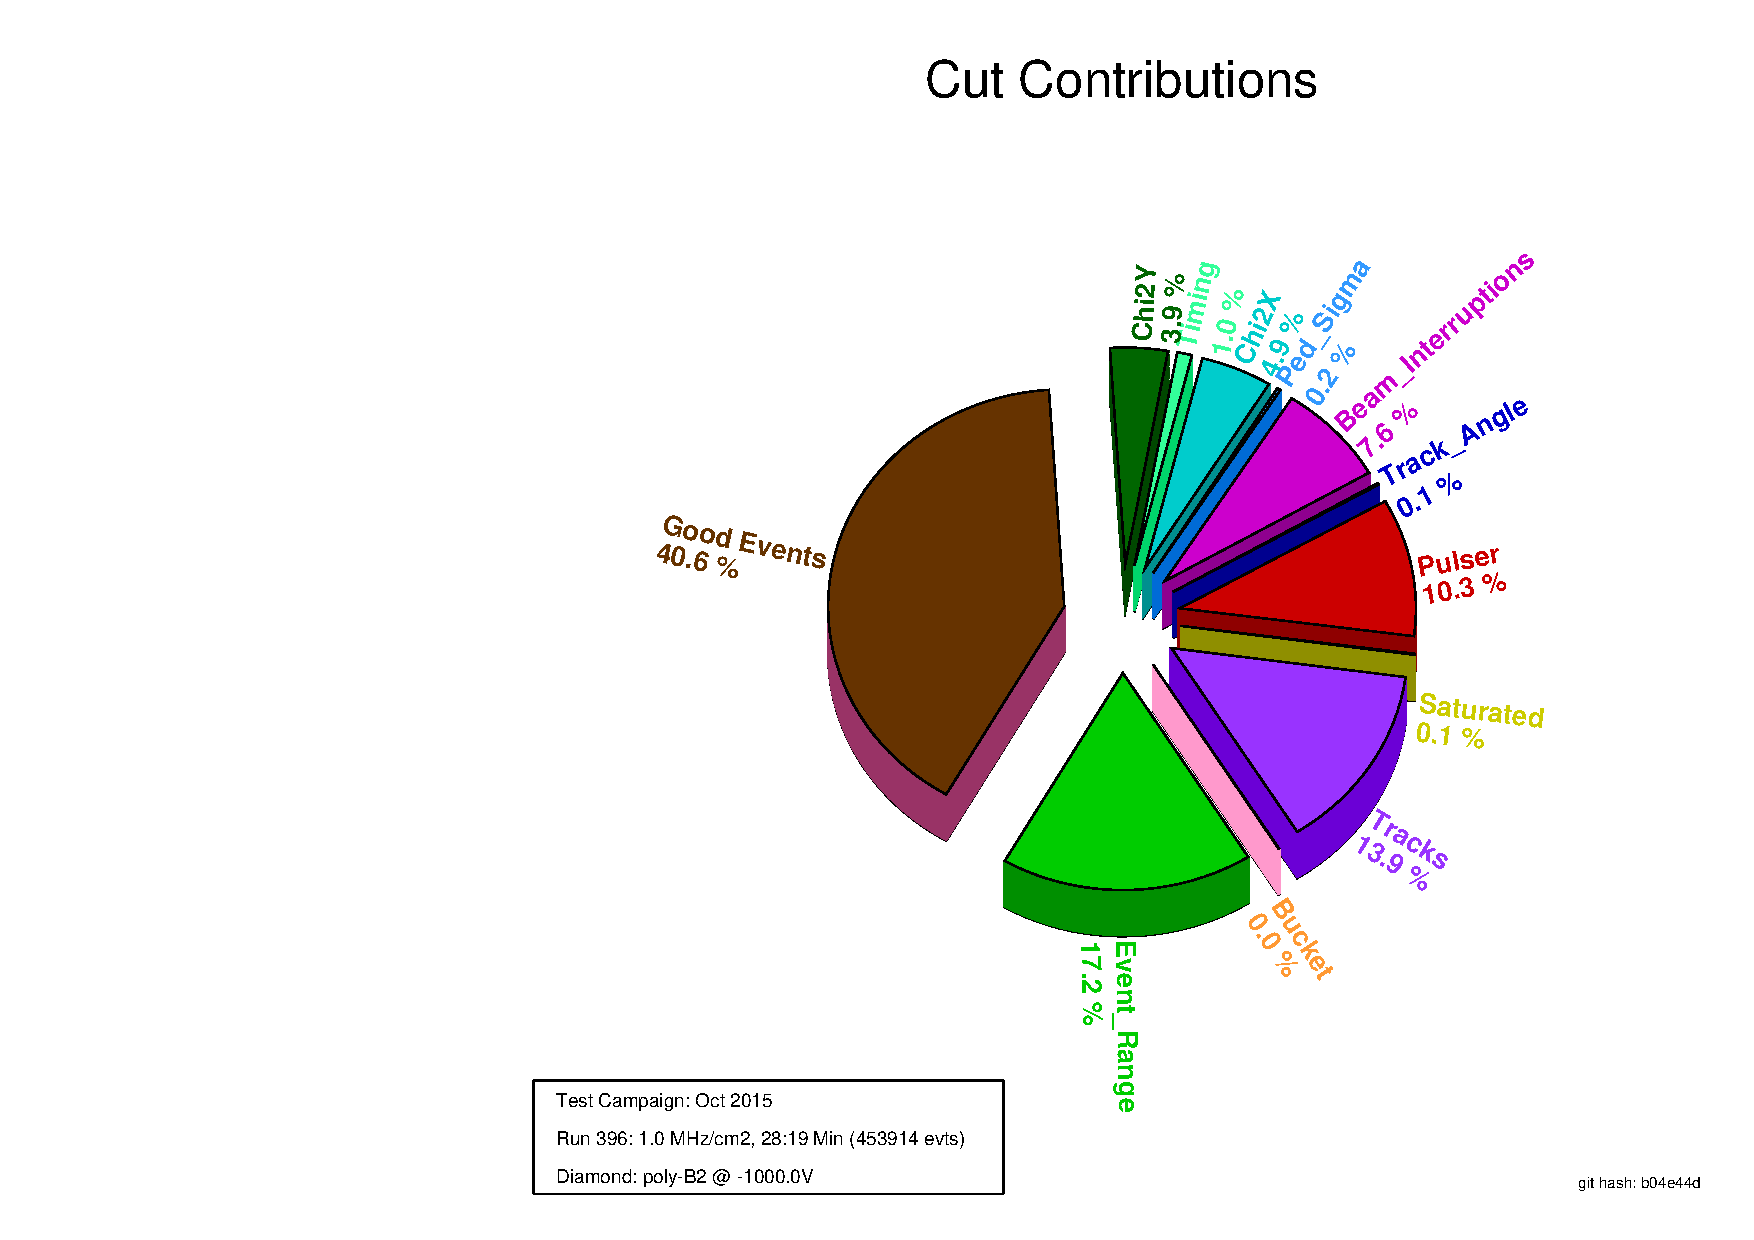
\includegraphics[angle=270, width=5.5cm]{CutContributions396}
	\end{minipage}
	\hspace*{2pt}
	\begin{minipage}{5.5cm}
		\centering
		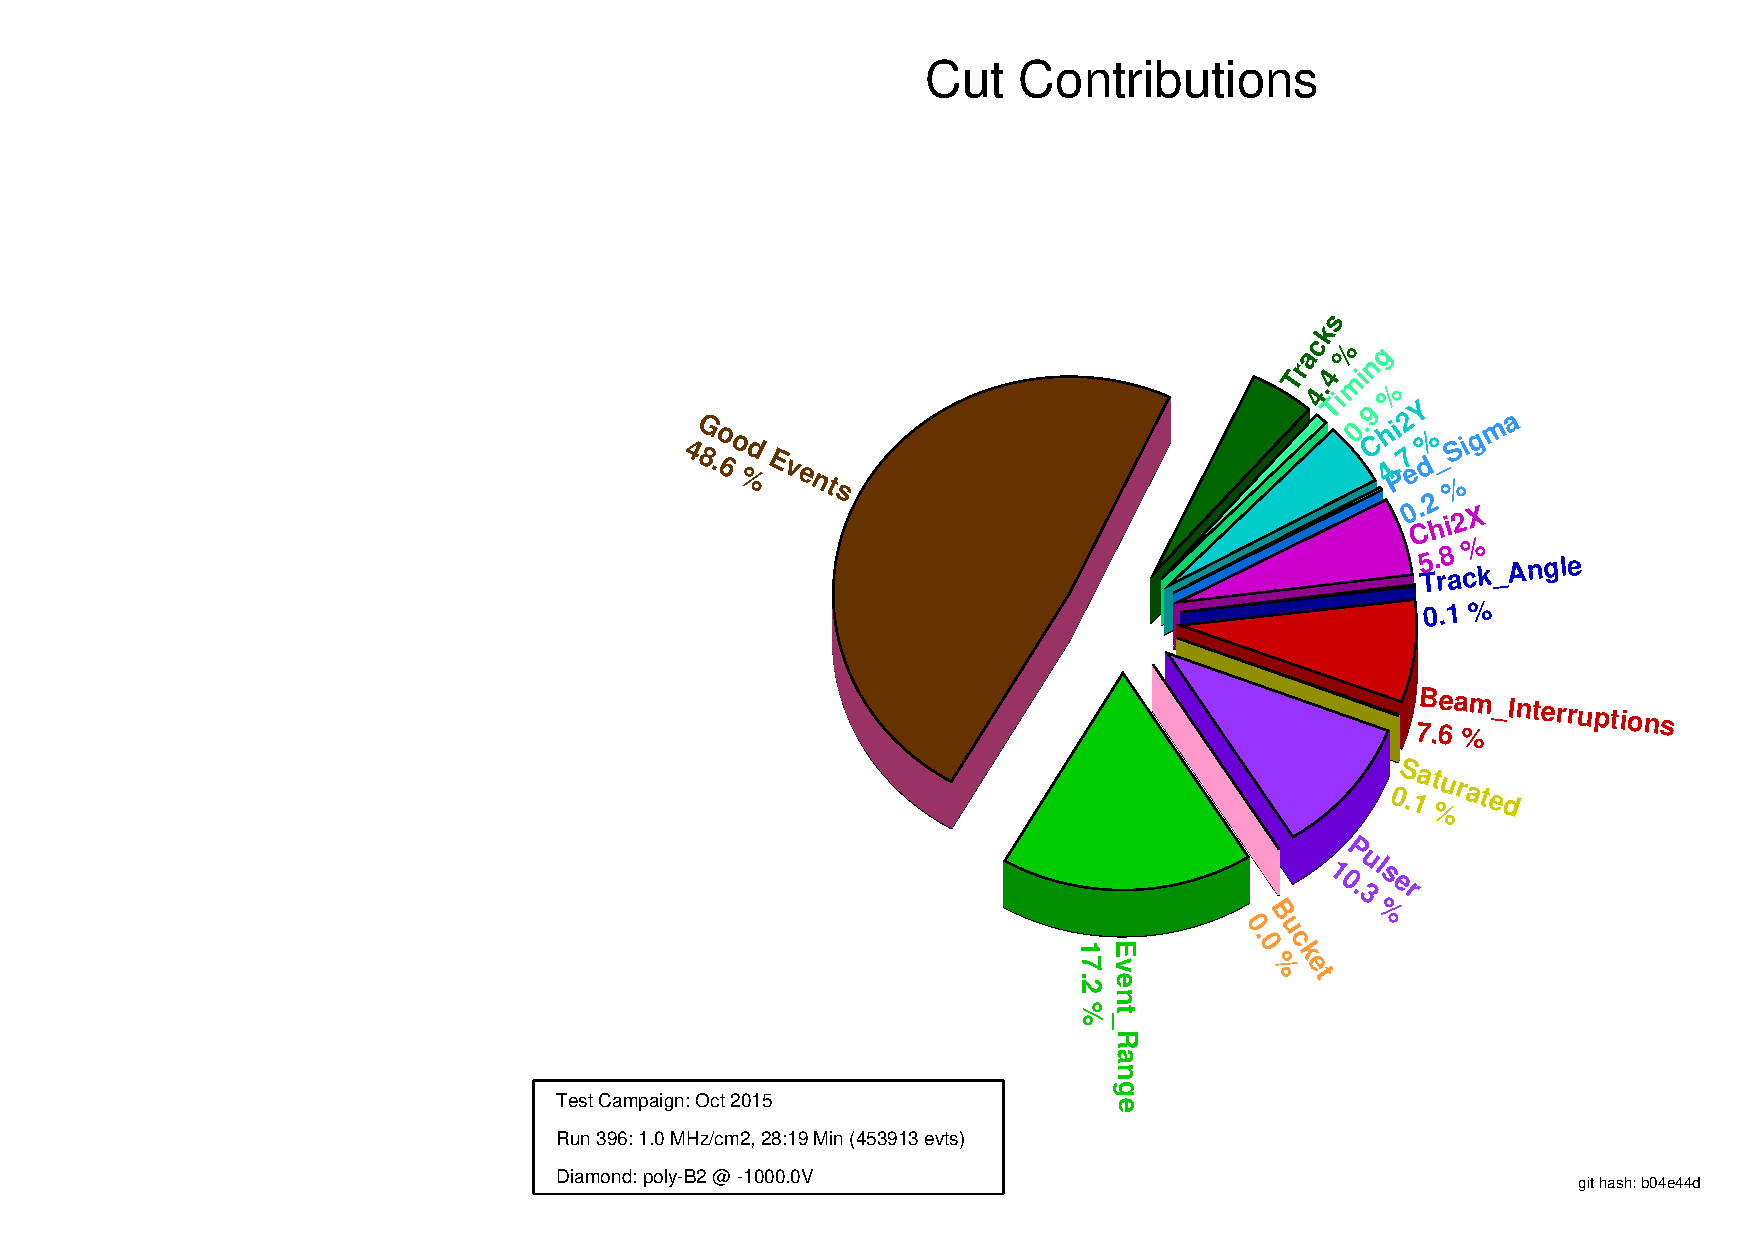
\includegraphics[angle=270, width=5.5cm]{CutContributions396a}
	\end{minipage}\s
\end{frame}
% END
% ====================================================================================
% BEGIN CONCLUSION
% ====================================================================================
\section{Conclusion}
% ============================
\begin{frame}
	\begin{minipage}[c][.5\textheight]{\textwidth}
		\begin{itemize}
			\setlength{\itemsep}{\fill}
			\item perhaps \SI{5}{\%} of the runs show an event misalignment right from the start
			\item misalignment weak influence on pulse height
			\item cut out wrong events
			\item working tool to correct for misalignment with negative offsets
		\end{itemize}
	\end{minipage}
\end{frame}
% END
% DOCUMENT END
\end{document}

